\documentclass{article}

%%%%
% babel
% PLOTS mapas y conglomerados
% bibliografia
%%%%
\usepackage{rotating}
\usepackage[utf8]{inputenc}
\usepackage{longtable}
\usepackage{authblk}
\usepackage{adjustbox}

\usepackage{natbib}

\usepackage[spanish]{babel}
\renewcommand\spanishtablename{Tabla}


\title{LOS INDICES DEL MUNDO}
% autores
\renewcommand\Authand{, y }
\author[1]{\normalsize Estrella DelCurso}
\author[2]{\normalsize Prossimo Deal Lado}

\affil[1,2]{\small  Escuela de Ingenier<U+00ED>a,Universidad de la vida\\
\texttt{{delcurso,deallado}@vida.edu}}
\affil[1]{\small Instituto de altas investigaciones financieras\\
Banco del Parque\\
\texttt{delcurso@bp.com}}

\date{}

%%%%
\usepackage{Sweave}
\begin{document}
\Sconcordance{concordance:paperVersion_6.tex:paperVersion_6.Rnw:%
1 34 1 1 0 26 1 1 6 3 1 1 12 42 0 1 2 11 1 1 35 1 2 6 1 1 7 12 0 1 2 1 %
7 15 0 1 2 5 1 1 8 13 0 1 2 7 1 1 8 11 0 1 2 6 1 1 4 1 2 11 1 1 5 1 1 1 %
3 37 0 1 2 12 1 1 9 1 1 1 23 5 1 1 20 1 2 8 1}


\maketitle


\begin{abstract}
Este es mi primer trabajo en exploracion y modelamiento de indices usando LATEX. Este trabajo lo he hecho bajo la filosof<U+00ED>a de trabajo replicable. Este es mi primer trabajo en exploracion y modelamiento de indices usando LATEX. Este trabajo lo he hecho bajo la filosof<U+00ED>a de trabajo replicable. Este es mi primer trabajo en exploracion y modelamiento de indices usando LATEX. Este trabajo lo he hecho bajo la filosof<U+00ED>a de trabajo replicable. Este es mi primer trabajo en exploracion y modelamiento de indices usando LATEX. Este trabajo lo he hecho bajo la filosof<U+00ED>a de trabajo replicable.
\end{abstract}

\section*{Introducci<U+00F3>n}

Aqui les presento mi investigacion sobre diversos indices sociales en el mundo. Los indices los consegu<U+00ED> de wikipedia, espero que les gusten mucho. Aqui les presento mi investigacion sobre diversos indices sociales en el mundo. Los indices los consegu<U+00ED> de wikipedia, espero que les gusten mucho.Aqui les presento mi investigacion sobre diversos indices sociales en el mundo. Los indices los consegu<U+00ED> de wikipedia, espero que les gusten mucho.Aqui les presento mi investigacion sobre diversos indices sociales en el mundo. Los indices los consegu<U+00ED> de wikipedia, espero que les gusten mucho.
Aqui les presento mi investigacion sobre diversos indices sociales en el mundo. Los indices los consegu<U+00ED> de wikipedia, espero que les gusten mucho.Aqui les presento mi investigacion sobre diversos indices sociales en el mundo. Los indices los consegu<U+00ED> de wikipedia, espero que les gusten mucho.Aqui les presento mi investigacion sobre diversos indices sociales en el mundo. Los indices los consegu<U+00ED> de wikipedia, espero que les gusten mucho.

Comencemos viendo que hay en la secci<U+00F3>n \ref{univariada} en la p<U+00E1>gina \pageref{univariada}.

\clearpage



\section{Exploraci<U+00F3>n Univariada}\label{univariada}

En esta secci<U+00F3>n exploro cada <U+00ED>ndice. En esta secci<U+00F3>n exploro cada <U+00ED>ndice. En esta secci<U+00F3>n exploro cada <U+00ED>ndice. En esta secci<U+00F3>n exploro cada <U+00ED>ndice. En esta secci<U+00F3>n exploro cada <U+00ED>ndice. En esta secci<U+00F3>n exploro cada <U+00ED>ndice. En esta secci<U+00F3>n exploro cada <U+00ED>ndice. En esta secci<U+00F3>n exploro cada <U+00ED>ndice. En esta secci<U+00F3>n exploro cada <U+00ED>ndice.





Para conocer el comportamiento de las variables se ha preparado la Tabla \ref{Tfrecuencias}, donde se describe la distribuci<U+00F3>n de las modalidades de cada variable. Los n<U+00FA>meros representan la situaci<U+00F3>n de algun pa<U+00ED>s en ese indicador, donde el mayor valor num<U+00E9>rico es la mejor situaci<U+00F3>n.

% latex table generated in R 3.3.3 by xtable 1.8-2 package
% Thu Aug  2 13:11:31 2018
\begingroup\normalsize
\begin{longtable}{llrrr}
\caption{Tablas de Frecuencia de la variables en estudio} \\ 
 \textbf{Variable} & \textbf{Levels} & $\mathbf{n}$ & $\mathbf{\%}$ & $\mathbf{\sum \%}$ \\ 
  \hline \hline
WorldFreedom & 1 very bad & 46 & 24.7 & 24.7 \\ 
   & 3 middle & 56 & 30.1 & 54.8 \\ 
   & 5 very good & 84 & 45.2 & 100.0 \\ 
   \hline
 & all & 186 & 100.0 &  \\ 
   \hline
\hline
EconomicFreedom & 1 very bad & 18 & 9.7 & 9.7 \\ 
   & 2 bad & 65 & 35.0 & 44.6 \\ 
   & 3 middle & 71 & 38.2 & 82.8 \\ 
   & 4 good & 26 & 14.0 & 96.8 \\ 
   & 5 very good & 6 & 3.2 & 100.0 \\ 
   \hline
 & all & 186 & 100.0 &  \\ 
   \hline
\hline
PressFreedom & 1 very bad & 20 & 10.8 & 10.8 \\ 
   & 2 bad & 44 & 23.7 & 34.4 \\ 
   & 3 middle & 60 & 32.3 & 66.7 \\ 
   & 4 good & 45 & 24.2 & 90.9 \\ 
   & 5 very good & 17 & 9.1 & 100.0 \\ 
   \hline
 & all & 186 & 100.0 &  \\ 
   \hline
\hline
Democracy & 1 very bad & 50 & 26.9 & 26.9 \\ 
   & 2 bad & 40 & 21.5 & 48.4 \\ 
   & 4 good & 77 & 41.4 & 89.8 \\ 
   & 5 very good & 19 & 10.2 & 100.0 \\ 
   \hline
 & all & 186 & 100.0 &  \\ 
   \hline
\hline
\hline
\label{Tfrecuencias}
\end{longtable}
\endgroup

Como apreciamos en la Tabla \ref{Tfrecuencias}, los pa<U+00ED>ses en la mejor situaci<U+00F3>n son los menos, salvo en el caso del \emph{<U+00ED>ndice de libertas mundial}\footnote{N<U+00F3>tese que esto se puede deber a la {\bf menor} cantidad de categor<U+00ED>as.}

\clearpage

Para resaltar lo anterior, tenemos la Figura \ref{barplots} en la p<U+00E1>gina \pageref{barplots}. 


%%%%% figure
\begin{figure}[h]
\centering
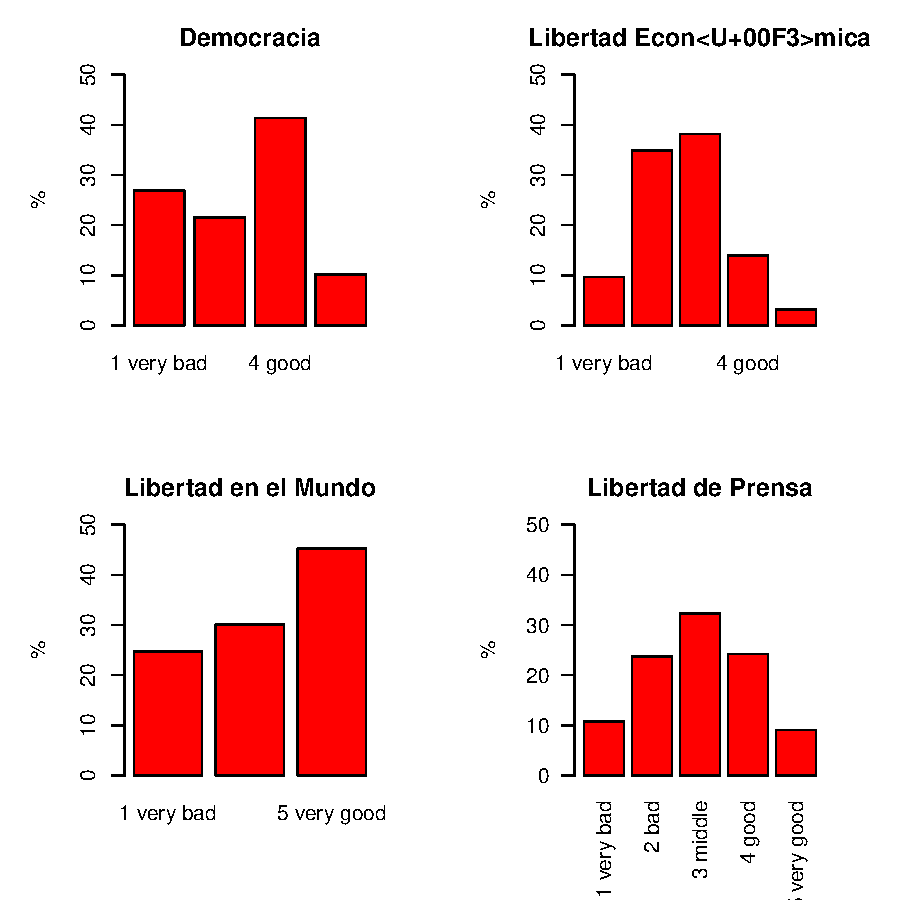
\includegraphics{paperVersion_6-barplots}
\caption{Distribuci<U+00F3>n de Indicadores}
\label{barplots}
\end{figure}

Adem<U+00E1>s de la distribuci<U+00F3>n de los variable, es importante saber el valor central y otros estad<U+00ED>sticos. La Tabla \ref{statsnum} de la p<U+00E1>gina \pageref{statsnum} y la Tabla \ref{statsord} de la p<U+00E1>gina \pageref{statsord} nos muestran los estad<U+00ED>sticos apropiados segun el tipo de variable.


% Table created by stargazer v.5.2.2 by Marek Hlavac, Harvard University. E-mail: hlavac at fas.harvard.edu
% Date and time: Thu, Aug 02, 2018 - 12:11:31
\begin{table}[!htbp] \centering 
  \caption{Estad<U+00ED>sticos para variables num<U+00E9>ricas} 
  \label{statsnum} 
\begin{tabular}{@{\extracolsep{5pt}}lccccc} 
\\[-1.8ex]\hline 
\hline \\[-1.8ex] 
Statistic & \multicolumn{1}{c}{N} & \multicolumn{1}{c}{Mean} & \multicolumn{1}{c}{Median} & \multicolumn{1}{c}{Min} & \multicolumn{1}{c}{Max} \\ 
\hline \\[-1.8ex] 
gdp & 186 & 21,667.200 & 13,000 & 700 & 139,100 \\ 
\hline \\[-1.8ex] 
\end{tabular} 
\end{table} 
% Table created by stargazer v.5.2.2 by Marek Hlavac, Harvard University. E-mail: hlavac at fas.harvard.edu
% Date and time: Thu, Aug 02, 2018 - 12:11:31
\begin{table}[!htbp] \centering 
  \caption{Estad<U+00ED>sticos para variables ordinales} 
  \label{statsord} 
\begin{tabular}{@{\extracolsep{5pt}}lcccc} 
\\[-1.8ex]\hline 
\hline \\[-1.8ex] 
Statistic & \multicolumn{1}{c}{N} & \multicolumn{1}{c}{Median} & \multicolumn{1}{c}{Max} & \multicolumn{1}{c}{Min} \\ 
\hline \\[-1.8ex] 
FreedomintheWorld & 186 & 3 & 5 & 1 \\ 
IndexofEconomicFreedom & 186 & 3 & 5 & 1 \\ 
PressFreedomIndex & 186 & 3 & 5 & 1 \\ 
DemocracyIndex & 186 & 4 & 5 & 1 \\ 
\hline \\[-1.8ex] 
\end{tabular} 
\end{table} 

\section{Exploraci<U+00F3>n Bivariada}

En este trabajo estamos interesados en el impacto de los otros indices en el nivel de Democracia. Veamos las relaciones bivariadas que tiene esta variable con todas las dem<U+00E1>s:

% Table created by stargazer v.5.2.2 by Marek Hlavac, Harvard University. E-mail: hlavac at fas.harvard.edu
% Date and time: Thu, Aug 02, 2018 - 12:11:31
\begin{table}[!htbp] \centering 
  \caption{Correlaci<U+00F3>n de GDP con las dem<U+00E1>s variables} 
  \label{corrDem} 
\begin{tabular}{@{\extracolsep{5pt}} cc} 
\\[-1.8ex]\hline 
\hline \\[-1.8ex] 
FreedomintheWorld & $0.247$ \\ 
IndexofEconomicFreedom & $0.588$ \\ 
PressFreedomIndex & $0.328$ \\ 
DemocracyIndex & $0.356$ \\ 
\hline \\[-1.8ex] 
\end{tabular} 
\end{table} 

Veamos la correlaci<U+00F3>n entre las variables independientes:


\begin{sidewaystable}
\centering
\caption{Correlaci<U+00F3>n entre variables independientes}
% Table created by stargazer v.5.2.2 by Marek Hlavac, Harvard University. E-mail: hlavac at fas.harvard.edu
% Date and time: Thu, Aug 02, 2018 - 12:11:31
\begin{tabular}{@{\extracolsep{5pt}} ccccc} 
\\[-1.8ex]\hline 
\hline \\[-1.8ex] 
 & FreedomintheWorld & IndexofEconomicFreedom & PressFreedomIndex & DemocracyIndex \\ 
\hline \\[-1.8ex] 
FreedomintheWorld & 1 &  &  &  \\ 
IndexofEconomicFreedom & 0.48 & 1 &  &  \\ 
PressFreedomIndex & 0.83 & 0.52 & 1 &  \\ 
DemocracyIndex & 0.89 & 0.58 & 0.76 & 1 \\ 
\hline \\[-1.8ex] 
\end{tabular} \end{sidewaystable}

Lo visto en la Tabla \ref{corrTableX} se refuerza claramente en la Figura \ref{corrPlotX}.

\begin{figure}[h]
\centering
\begin{adjustbox}{width=7cm,height=7cm,clip,trim=1.5cm 0.5cm 0cm 1.5cm}
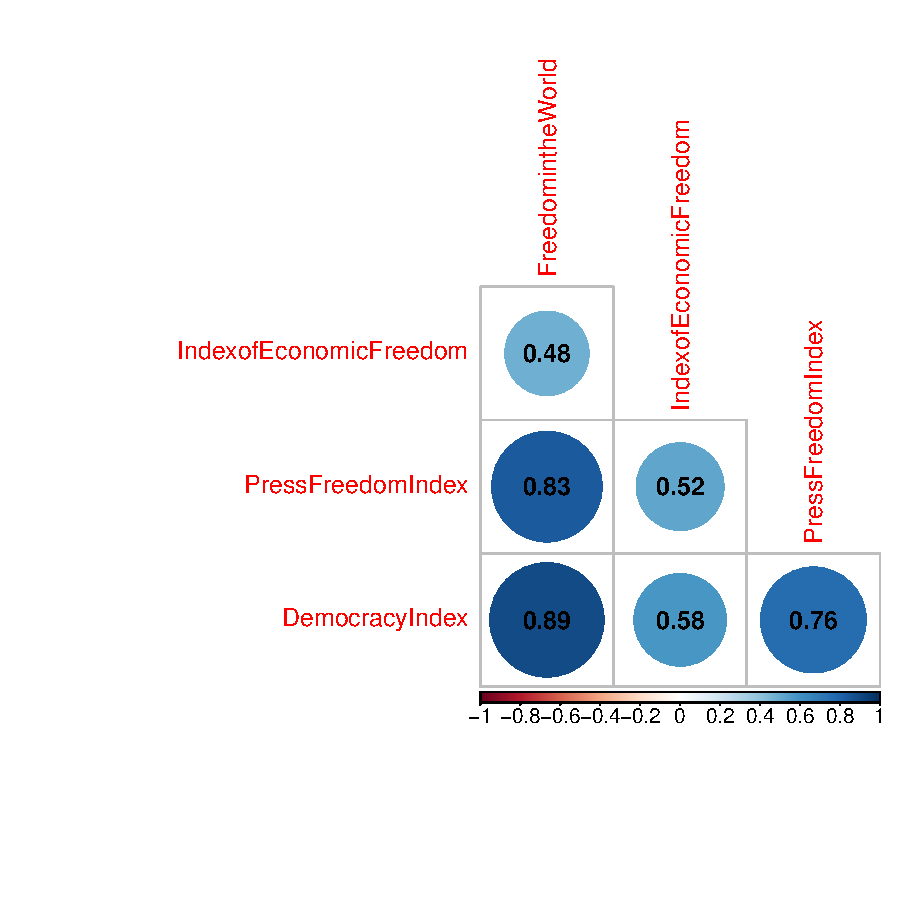
\includegraphics{paperVersion_6-corrPlotX}
\end{adjustbox}
\caption{correlaci<U+00F3>n entre predictores}
\label{corrPlotX}
\end{figure}


\clearpage

\section{Modelos de Regresi<U+00F3>n}

FFinalmente, vemos los modelos propuestos. Primero sin el <U+00ED>ndice de democracia como independiente, y luego con <U+00E9>ste. Los resultados se muestran en la Tabla \ref{regresiones} de la p<U+00E1>gina \pageref{regresiones}.



% Table created by stargazer v.5.2.2 by Marek Hlavac, Harvard University. E-mail: hlavac at fas.harvard.edu
% Date and time: Thu, Aug 02, 2018 - 12:11:31
\begin{table}[!htbp] \centering 
  \caption{Modelos de Regresi<U+00F3>n} 
  \label{regresiones} 
\begin{tabular}{@{\extracolsep{5pt}}lcc} 
\\[-1.8ex]\hline 
\hline \\[-1.8ex] 
 & \multicolumn{2}{c}{\textit{Dependent variable:}} \\ 
\cline{2-3} 
\\[-1.8ex] & \multicolumn{2}{c}{gdp} \\ 
\\[-1.8ex] & (1) & (2)\\ 
\hline \\[-1.8ex] 
 FreedomintheWorld & $-$2,582.285 & $-$5,505.874$^{**}$ \\ 
  & (1,579.153) & (2,305.879) \\ 
  & & \\ 
 IndexofEconomicFreedom & 14,823.900$^{***}$ & 13,575.000$^{***}$ \\ 
  & (1,779.269) & (1,910.907) \\ 
  & & \\ 
 PressFreedomIndex & 3,569.733 & 3,570.992 \\ 
  & (2,326.908) & (2,314.236) \\ 
  & & \\ 
 DemocracyIndex &  & 4,103.246$^{*}$ \\ 
  &  & (2,369.556) \\ 
  & & \\ 
 Constant & $-$19,594.750$^{***}$ & $-$18,067.700$^{***}$ \\ 
  & (4,707.167) & (4,763.864) \\ 
  & & \\ 
\hline \\[-1.8ex] 
Observations & 186 & 186 \\ 
R$^{2}$ & 0.355 & 0.366 \\ 
Adjusted R$^{2}$ & 0.345 & 0.352 \\ 
Residual Std. Error & 19,424.840 (df = 182) & 19,319.060 (df = 181) \\ 
F Statistic & 33.455$^{***}$ (df = 3; 182) & 26.117$^{***}$ (df = 4; 181) \\ 
\hline 
\hline \\[-1.8ex] 
\textit{Note:}  & \multicolumn{2}{r}{$^{*}$p$<$0.1; $^{**}$p$<$0.05; $^{***}$p$<$0.01} \\ 
\end{tabular} 
\end{table} 
\clearpage

\section{Exploraci<U+00F3>n Espacial}

Como acabamos de ver en la Tabla \ref{regresiones} en la p<U+00E1>gina \pageref{regresiones}, si quisieras sintetizar la multidimensionalidad de nuestros indicadores, podr<U+00ED>amos usar las cuatro variables ordinales que tenemos. 

As<U+00ED>, propongo que calculemos conglomerados de pa<U+00ED>ses usando toda la informaci<U+00F3>n de esos indicadores. Como estas variables son ordinales, utilizaremos un proceso de conglomeraci<U+00F3>n donde las distancia ser<U+00E1>n calculadas usando la medida {\bf gower} 
propuesta por \cite{gower_general_1971}
, y para los enlazamientos usaremos la t<U+00E9>cnica de {\bf medoides} 
siguiendo a \cite{reynolds_clustering_2006}
. Los tres conglomerados se muestran en la Figura \ref{clustmap}.






\begin{figure}[h]
\centering
\begin{adjustbox}{width=11cm,height=8cm,clip,trim=1cm 2.5cm 0cm 2.5cm}
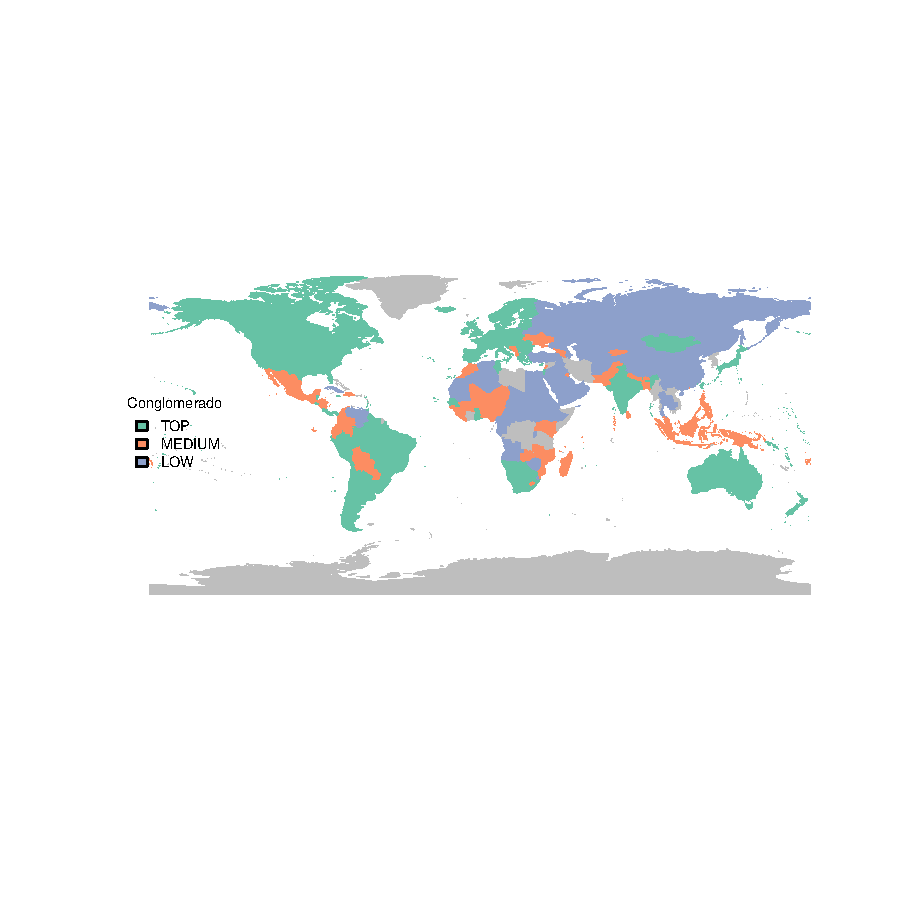
\includegraphics{paperVersion_6-plotMap1}
\end{adjustbox}
\caption{Paises conglomerados segun sus indicadores sociopol<U+00ED>ticos}\label{clustmap}
\end{figure}

\bibliographystyle{apalike}
% \renewcommand{\refname}{Bibliografia}
\bibliography{biblio}

\end{document}
